\documentclass[a4paper, english, 12pt, hidelinks]{article}
\usepackage[a4paper, top=2cm, bottom=2cm, left=2cm, right=2cm]{geometry}
\usepackage[english]{babel}
\usepackage[utf8]{inputenc}
\usepackage{float}
\usepackage{subfig}
\usepackage[table]{xcolor}		% Fargede tabeller
\usepackage{tabularx}
\usepackage{graphicx}
\usepackage{transparent}
\usepackage{footnote}
% \usepackage{perpage} 			% For å få fotnotenummerering til å starte på nytt for hver side
% \usepackage[bottom]{footmisc}	% Footnotes på sideslutt
\usepackage[parfill]{parskip}	% Linjeskift istedetfor tabbing
%\usepackage{fancyhdr}	        % Headerpå alle sider
\usepackage{fix-cm}	            % stor skrift
\renewcommand*{\familydefault}{\sfdefault}
\usepackage{epsf} 
\usepackage{eso-pic}
\usepackage{wrapfig}        % Tables inline with text
\usepackage{hyperref}       % Links
\usepackage{longtable}

\definecolor{dkgreen}{rgb}{0,0.6,0}	    % For kildekode
\definecolor{gray}{rgb}{0.5,0.5,0.5}
\definecolor{mauve}{rgb}{0.58,0,0.82}
\definecolor{light-gray}{gray}{0.95}	% For tabeller
\definecolor{medium-gray}{gray}{0.5}	% For tabeller
\definecolor{dark-gray}{gray}{0.3}	    % For tabeller
\definecolor{to-radio}{rgb}{0.8,0.2,0.2}
\definecolor{from-radio}{rgb}{0.1,0.5,0.1}
% \MakePerPage{footnote} % For å få fotnotenummerering til å starte på nytt for hver side
\newcommand{\HRule}{\rule{\linewidth}{0.5mm}}
\def\arraystretch{1.3} % Table padding!

\begin{document}

% Front page
\begin{titlepage}

    \begin{centering}
\topskip0pt
\vspace*{\fill}
	    {\color{medium-gray}\HRule}
	    \\[0.6cm]
	    \color{dark-gray}
	    \fontsize{50}{40}{\selectfont NGHam}
        \\[0.2cm]
	    \fontsize{16}{20}{\selectfont Packet Radio Protocol}
        \\[0.2cm]
	    \fontsize{14}{20}{Revision C, \today, \url{http://github.com/skagmo/ngham/}}
        \\[0.2cm]
	    {\color{medium-gray}\HRule}
\vspace*{\fill}
    \end{centering}
\end{titlepage}

\tableofcontents
\clearpage

% Spec. list
\section{Introduction}
    NGHam is a protocol set for packet based amateur radio, intended to resolve some issues with
    currently used protocols AX.25 and KISS. Its key features are:

    \begin{description}
        \item[Very robust:] Allows decoding with much lower SNR compared to 1200 baud AFSK AX.25 due to the 
        use of a sync word with good autocorrelation properties and Reed Solomon FEC over the whole
        remaining packet.
        \item[High throughput:] Due to the short preamble and increased chance of successful packet reception,
        the practical throughput will be much higher than when using AX.25.
        \item[Better spectral efficiency:] Significantly better spectral efficiency than 1200 baud AFSK, and
        somewhat better than 9600 baud G3RUH modulation due to the reduced deviation.
    \end{description}

    NGHam can be divided into three sub-protocols: NGHam RF, SPP (Serial Port Protocol) and Extension.
    \\[0.2cm]
    \begin{figure}[H]
	    \centering
	    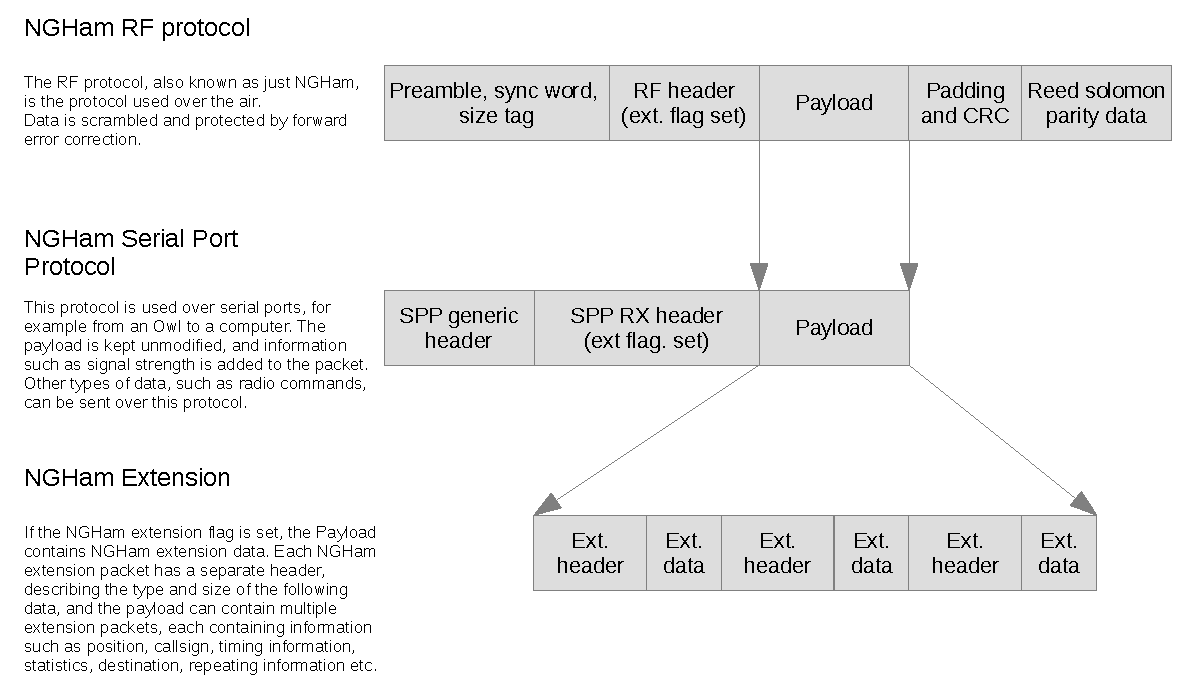
\includegraphics[width = \textwidth, trim=0cm 0cm 0cm 0cm, clip]{img/ngham_protocol_stack.pdf}
	    \caption{NGHam protocol stack}
	    \label{fig:ngham_stack}
    \end{figure}

	\clearpage

\section{Radio Protocol}
    The structure of an NGHam radio packet is shown below.

    \begin{figure}[H]
	    \centering
	    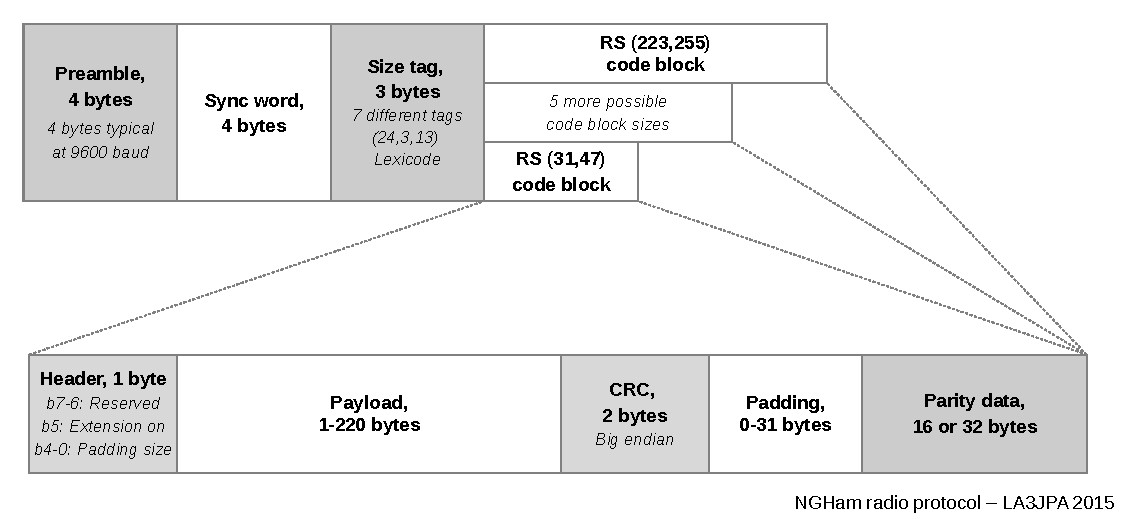
\includegraphics[width = \textwidth, trim=0cm 0cm 0cm 0cm, clip]{img/ngham_block_v4.pdf}
	    \caption{NGHam RF packet}
	    \label{fig:ngham_rf_packet}
    \end{figure}

    \begin{description}
        \item[Preamble:] The preamble is short, and is transmitted while the PA is ramping up and the receiver AGC
        is stabilizing. Will vary with symbol rate, but 4 bytes is typically used for 9600 baud.
        Sync word for bit- and packet-synchronization: A 32-bit correlation tag / sync word allows both bit-
        synchronization and detection of packet start in very short time and in very low S/N conditions. This
        means the preamble can be drastically reduced from the order of 100 ms as we typically see for
        AX.25 today, down to under 5 ms - depending on how fast the hardware can switch to transmission.
        This also increases the chance of detecting the packet start substantially.

        \item[Size tag:] A 24 bit tag identifies one out of 7 possible code word sizes. This is made very robust by
        keeping a hamming distance of 13 bits between all vectors.

        \item[Code block:] NGHam uses Reed Solomon block error correction to make it robust against bursts of
        errors. NGHam has no inner convolutional error correction, and this was decided to increase
        throughput at the cost of a somewhat higher SNR margin. Reed Solomon is a robust error correction
        scheme with no restrictions on usage (as opposed to eg. many turbo codes), and Phil Karn, KA9Q,
        provides an open source C-implementation with LGPL licensing (\url{http://www.ka9q.net/code/fec/}).
        Reed Solomon has a fixed block size, so some different methods for allowing variable packet sizes were evaluated.
        Initially a preceding 12 bit length field with a (12,24) golay FEC allowing a variable
        packet length down to a single byte was tested, but this turned out to reduce the robustness due to
        it only being capable of correcting single bit errors. The final solution was to allow seven differently
        sized code blocks identified by a size tag. The transmitter chooses the smallest code block that can fit
        the payload to be sent, and the remaining bytes are padded. This allows higher robustness than the
        first method at a cost of a 0-31 byte overhead.

        \item[Scrambling:] K9NG polynomial scrambling has served well for 9k6 AX.25 packet in many years, but
        unfortunately it cannot be used with most FEC-schemes as errors propagate throughout the packet.
        XOR-ing the data with a fixed sequence at encoding and decoding allows zero delay, synchronization
        with packet start, and no propagating errors. The polynomial used for generating the table is x\^{}8 +
        x\^{}7 + x\^{}5 + x\^{}3 + 1 (as of CCSDS 101.0-B-3).

        \item[Modulation:] GMSK modulation with bt=0.5 should be used. 9600 baud 2-GMSK is the default rate,
        but combinations of 4800, 9600 and 19200 baud symbol rate at 2-GMSK and 4-GMSK are all valid. At
        4-GMSK the preamble and sync word should be transmitted using 2-GMSK.

        \item[Channel access:] Due to the very different uses, CSMA should work as the default access scheme.
        However, the channel access could be changed depending on the next layer protocol. For example, a
        positioning protocol with regular short transmissions of pretty much the same length, such as APRS,
        should use a TDMA-derived scheme. This will allow a lot more efficient channel usage than when using CSMA.
        For transferring bigger amounts of data between a few people, a MACA-scheme with RTS/CTS
        packets as described by Phil Karn could be the most efficient method, but none of this is
        implemented as of today.

        \item[Continous transmission:] All NGHam devices should supports continuous transmission and reception
        (ring buffers are used where needed) by stacking packets end-to-end.
    \end{description}
	\clearpage

\section{Serial Port Protocol}
    This chapter describes the protocol used to transfer data and commands between the transceiver
    and the serial port host.

    \subsection{General format}
		\begin{table}[H]
			\centering
			\rowcolors{2}{}{light-gray}
			\begin{tabular}{|p{3cm}|p{2cm}|p{10cm}|}
				\hline
				Name & Size (Byte) & Notes \\
				\hline
                Start tag & 1 & Fixed as '\$'. \\
                CRC Size & 2 & 16-bit CRC CCITT (start=0xffff, polynomial=0x1021 reversed, Xorout=0xffff). 
                Notice the use of little endian, as everything on this layer and up use little endian.
                CRC is calculated of everything except start tag and CRC itself.\\
                Payload type & 1 & 0x00=RF receive packet, 0x01=RF transmit packet, 0x02=Local packet, 0x03=Command. \\
                Payload length & 1 & Length of payload field. \\
                Payload & n & This is the actual payload specified by the payload type. \\
				\hline
			\end{tabular}
		\end{table}

    \subsection{Type RF receive packet (from radio to host)}
        Data received from RF link. Length from 4 to 223. The table below describes what is put into the
        payload of the general packet format.
		\begin{table}[H]
			\centering
			\rowcolors{2}{}{light-gray}
			\begin{tabular}{|p{3cm}|p{2cm}|p{10cm}|}
				\hline
				Name & Size (Byte) & Notes \\
				\hline
                Time of hour in microseconds & 4 & Local time of hour timestamp of the incoming packet. 
                Wraps from 3599999999 (one step before 3600 seconds) to 0. N/A-value is 0xffffffff. \\          
                Noise floor & 1 & Subtract 200 to get dBm. Eg. 0x50 = -120 dBm. N/A-value is 0xff. \\
                RSSI & 1 & Same as above. \\
                Symbol errors & 1 & Number of corrected Reed Solomon symbols. \\
                Flags & 1 & Bit 0: NGHam extension enabled. If this bit is set, the data field is a valid NGHam extension packet.  \\
                Data & n-8 B & Received data. \\
				\hline
			\end{tabular}
		\end{table}

    \subsection{Type RF transmit packet (from host to radio)}
        Data to be transmitted on RF link. Length from 1 to 220. The table below describes what is 
        put into the payload of the general packet format.
		\begin{table}[H]
			\centering
			\rowcolors{2}{}{light-gray}
			\begin{tabular}{|p{3cm}|p{2cm}|p{10cm}|}
				\hline
				Name & Size (Byte) & Notes \\
				\hline
                Flags & 1 & Bit 0: NGHam extension enabled flag. \\
                Data & n-1 B & Data to be transmitted. \\
				\hline
			\end{tabular}
		\end{table}

    \subsection{Type local packet (from radio to host)}
        Packet generated by the radio (not received over the air). For example a status report. The table below describes what is 
        put into the payload of the general packet format.
		\begin{table}[H]
			\centering
			\rowcolors{2}{}{light-gray}
			\begin{tabular}{|p{3cm}|p{2cm}|p{10cm}|}
				\hline
				Name & Size (Byte) & Notes \\
				\hline
                Flags & 1 & Bit 0: NGHam extension enabled flag. \\
                Data & n-1 B & Data to be transmitted. \\
				\hline
			\end{tabular}
		\end{table}

    \subsection{Type CMD}
        This type of packet is used to enter commands. On the Owl VHF, this command will do the same as 
        typing into the command-line interpreter, except the commands and replies are not terminated by LF/CR/CRLF. 
        The table below describes what is put into the payload of the general packet format.
		\begin{table}[H]
			\centering
			\rowcolors{2}{}{light-gray}
			\begin{tabular}{|p{3cm}|p{2cm}|p{10cm}|}
				\hline
				Name & Size (Byte) & Notes \\
				\hline
                Command & n B & Non-terminated command, as for example "FREQ 144800000". \\
				\hline
			\end{tabular}
		\end{table}

\end{document}
